%%%%%%%%%%%%%%%%%%%%%%%%%%%%%%%%%%%%%%%%%%%%%%%%%%%%%%%%%%%%%%%%%%%%%%%%%%%%%%%%
% Author : David Cislak
% Description : Seventh exercise in the Introduction to Game Development course.
%   It deals with the creation of a Game Design Document, presenting a short 
%   pitch for a potential game project.
%%%%%%%%%%%%%%%%%%%%%%%%%%%%%%%%%%%%%%%%%%%%%%%%%%%%%%%%%%%%%%%%%%%%%%%%%%%%%%%%

\documentclass[a4paper,10pt,english]{article}

\usepackage[left=2.50cm,right=2.50cm,top=1.50cm,bottom=2.50cm]{geometry}
\usepackage[utf8]{inputenc}

% Hyper-Text References
\usepackage{hyperref}
\hypersetup{colorlinks=true, urlcolor=blue}

% Drawing Images and Graphs
\usepackage{tikz}
\usepackage{pgfplots}

% Page Utilities
\usepackage{graphicx}

% Image Sub-Captions
\usepackage{subcaption}

\newcommand{\ph}[1]{\textit{[#1]}}

\title{%
Game Pitch Document%
}
\author{%
Dávid Čislák (xcislad00)%
}
\date{}

\begin{document}

\maketitle
\thispagestyle{empty}

{%
\large

\begin{itemize}

\item[] \textbf{Title:} Steel Tomb

\item[] \textbf{Genre:} First-Person, Survival Horror / Simulation

\item[] \textbf{Style:} 3D, Semi-Realistic, Industrial, Claustrophobic

\item[] \textbf{Platform:} PC (Mouse/Keyboard), VR (Potential)

\item[] \textbf{Market:} Individuals interested in war, tanks and horror games like \textbf{Iron Lung} or \textbf{Amnesia}

\item[] \textbf{Elevator Pitch:} Trapped in a tank with a dead crew, you must operate internal systems and rely on limited audio-visual cues to survive whatever dangers await you

\end{itemize}

}

\section*{\centering The Pitch}

\subsection*{Introduction}
\textbf{Steel Tomb} is a claustrophobic survival simulation. Unlike shooters, where combat is external and visual, this game focuses on internal operation of a heavy tank, where the player, trapped with a deceased crew, must rely on limited audio and visual feedback to navigate hostile enviroment. 

\subsection*{Background}
\emph{War Thunder} and its realism are the main source of inspiration for this game. Complex manual interactions build upon the sensory deprivation mechanics found in a game like \textit{Iron Lung} and enhance it. The primary objective is to strip the player of "power fantasy" of driving a powerfull tank, replacing it with a feeling of being trapped inside of a metal box.

\subsection*{Setting}
The narrative takes place within an imaginary tank "T-56B" during a late–Cold War border conflict, sometime in the early 1960s. The player awakens alone inside a disabled Soviet T-56B tank after an engagement has ended. The player is the tanks only survivor, the original crew is dead, their bodies still occupying stations, forcing the player to operate the tank, while moving around them. 

\subsection*{Features}
\begin{itemize}
    \item Historical Aesthetic
    
    Inspired by late–Cold War Soviet engineering, the game avoids advanced graphics or futuristic elements, appealing to players who value realism, and atmosphere of games the most.

    \item Sensory Deprivation–Driven Tension

    Limited visibility and audio, unreliable machinery, and environmental noise build tension through uncertainty and interpretation.

    \item Manual, Mechanical Interaction
    
    All core actions—turret rotation, engine startup etc. are performed through hand-cranked, analog systems. This emphasizes physical effort, prediction and synchronization with sensory elements over reflexes or automation.
    
\end{itemize}

\begin{figure}[h]

\centering
    
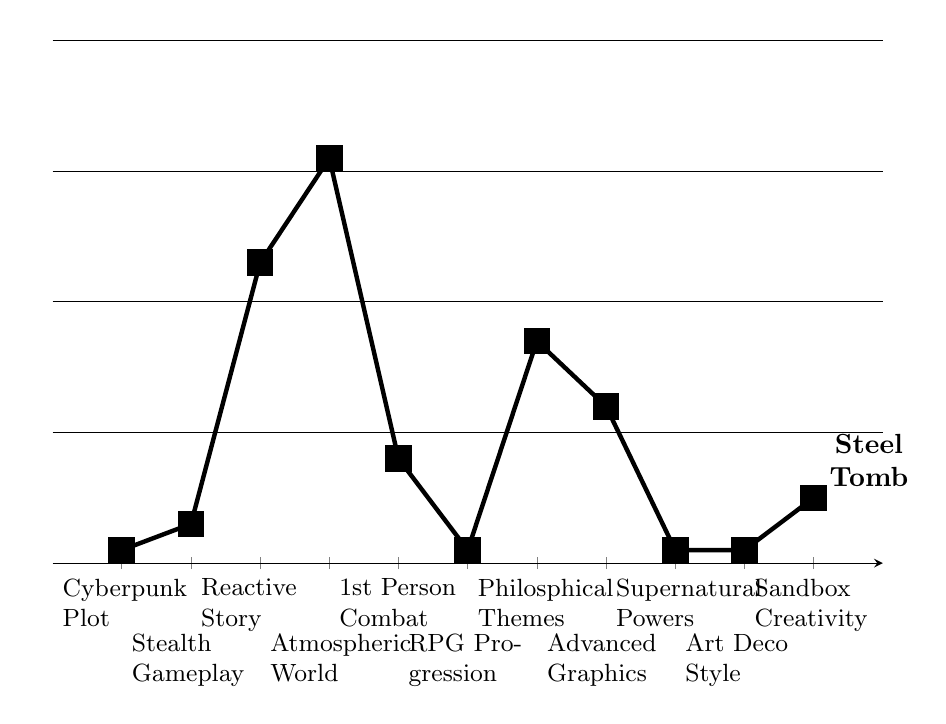
\begin{tikzpicture}[remember picture]%
\begin{axis}[
    domain=0:1, 
    clip=false, 
    ymin=0, xmin=0, ymax=4.1, xmax=12, 
    xtick={1,2,...,11}, 
    yticklabels={}, 
    xticklabels={Cyberpunk Plot, Stealth Gameplay, Reactive Story, Atmospheric World, 1st Person Combat, RPG Progression, Philosphical Themes, Advanced Graphics, Supernatural Powers, Art Deco Style, Sandbox Creativity}, 
    xticklabel style={yshift={-mod(\ticknum, 2) * 2em}, text width=1.5cm, font=\small}, 
    y tick style={draw=none}, 
    x axis line style={|-|}, 
    y axis line style={draw=none}, 
    axis lines=middle, 
    width=\linewidth, 
    height=0.3\paperheight
]
        \addplot [ultra thick, mark=square*, mark options={scale=2,solid}] coordinates {
        (1, 0.1)
        (2, 0.3)
        (3, 2.3)
        (4, 3.1)
        (5, 0.8)
        (6, 0.1)
        (7, 1.7)
        (8, 1.2)
        (9, 0.1)
        (10, 0.1)
        (11, 0.5)
    } node[above, yshift=0pt, xshift=20pt, pos=1, text width=1cm, align=center] {\textbf{Steel Tomb}};
    
	\draw [] (axis cs:{0,1}) -- (axis cs:{12,1});
	\draw [] (axis cs:{0,2}) -- (axis cs:{12,2});
	\draw [] (axis cs:{0,3}) -- (axis cs:{12,3});
	\draw [] (axis cs:{0,4}) -- (axis cs:{12,4});
\end{axis}
\end{tikzpicture}

\caption{Value graph for \emph{Steel Tomb}.}
\label{Fig:ValueGraph}

\end{figure}

\subsection*{Genre}
While someone could say, that the game is technically a \textbf{Vehicle Simulation}, the game diverges significantly by employing the pacing and tension of \textbf{Survival Horror}. It is meant to act as a deconstruction of the war-game fantasy and puts emphasis on the human cost of warfare.

\subsection*{Platform}
Steel Tomb is primarily designed for PC, which serves as the core platform due to its support for complex input schemes. A potential VR version is planned as well, focusing on the game’s first-person perspective and physical interactions to enhance immersion and claustrophobia.

\subsection*{Style}

\begin{figure}[htbp]
\centering
\includegraphics[width=\linewidth]{tank_xray.png}
\caption{Tank x-ray}
\label{Fig:Style1A}
\end{figure}

\begin{figure}[htbp]
\centering
\includegraphics[width=\linewidth]{metro2033.png}
\caption{Style of the potential environment and user interface}
\label{Fig:Style1B}
\end{figure}

\begin{figure}[htbp]
\centering
\includegraphics[width=\linewidth]{Iron_Lung.png}
\caption{Different gauges and levers for manual control}
\label{Fig:Style1C}
\end{figure}



\end{document}
